\documentclass[12pt]{article}
\usepackage{epsfig}
\usepackage{natbib}
\usepackage{color}
\usepackage{graphicx}
\usepackage{amssymb,amsmath}

\definecolor{orange}{cmyk}{0,0.4,0.8,0.2}
\definecolor{darkorange}{rgb}{.71,0.21,0.01}
\definecolor{darkgreen}{rgb}{.12,.54,.11}
\definecolor{darkblue}{rgb}{0.1,0.1,0.8}
\usepackage{hyperref}
\hypersetup{pdftex,  % needed for pdflatex
  breaklinks=true,  % so long urls are correctly broken across lines
  colorlinks=true,
  urlcolor=blue,
  linkcolor=darkorange,
  citecolor=darkgreen,
  }

\pagestyle{plain}
\topmargin 0in
\headheight 0in
\headsep 0in
\footskip 0.5in

\textheight 9.0in
%\textwidth 6.7in
\textwidth 6.5in

\oddsidemargin 0in
\evensidemargin 0in
\marginparwidth 0in
\baselineskip0.2cm
\parskip0.1cm
\font\cap=cmcsc10

\def\ni{\noindent}        %No Indent%
\def\ub{\underbar}
\def\hi{\noindent \hangindent=2.5em}
\def\et{{\it et\thinspace al.}}    %et al.%
\def\hour{^{\rm h}}
\def\minute{^{\rm m}}
\def\second{^{\rm s}}
\def\arcmin{^{\prime}}
\def\arcsec{^{\prime\prime}}
\def\pixel{{\rm\,pixel}}
\def\degrees{{\rm\,degrees}}
\def\pc{{\rm\,pc}}
\def\cm{{\rm\,cm}}
\def\kms{{\rm\,km/s}}
\def\kpc{{\rm\,kpc}}
\def\hkpc{{\rm\,$h_{50}^{-1}$\,kpc}}
\def\hpc{{\rm\,$h_{50}^{-1}$\,pc}}
\def\Mpc{{\rm\,Mpc}}
\def\mpc{{\rm\,Mpc}}
\def\Gyr{{\rm\,Gyr}}
\def\kmsec{{\rm\,km/s}}
\def\hnot{{\rm\,km/s/Mpc}}
\def\msun{{\rm\,M_\odot}}
\def\lsun{{\rm\,L_\odot}}
\def\mdot{{\rm\,M_\odot}}
\def\surfb{{\rm\,mag/arcsec^2}}
\def\araa{{\it Ann.\ Rev.\ Astr.\ Ap.}}
\def\actaa{{\it Acta~Astronomica}}
\def\aj{{\it A.~J.}}  %Astronomical Journal%
\def\apj{{\it Ap.~J.}}  %Astrophysical Journal%
\def\apjs{{\it Ap.~J.~Suppl.}}  %Astrophysical Journal Supplements%
\def\apjl{{\it Ap.~J.~(Letters)}} %Astrophysical Journal Letters%
\def\pasp{{\it Pub.~A.S.P.}}      %Publications of the Astronomical%
                                %Society of the Pacific%
\def\memsai{{\it Memorie della Societ� Astronomica Italiana}}
\def\mn{{\it M.N.R.A.S.}}      %Monthly Notices of the Royal%
                                %Astronomical Society%
\def\mnras{{\it M.N.R.A.S.}}      %Monthly Notices of the Royal%
                                %Astronomical Society%
\def\nat{{\it Nature}}      %Nature%
\def\aa{{\it Astr.~Ap.}}     %Astronomy & Astrophysics%
\def\aap{{\it Astr.~Ap.}}     %Astronomy & Astrophysics%
\def\aasup{{\it Astr.~Ap.~Suppl.}}     %A & A Supplements%
\def\aaps{{\it Astr.~Ap.~Suppl.}}     %A & A Supplements%
\def\ass{{\it Astr.~Sp.~Sci.}}     %A & A Supplements%
\def\ssr{{\it Space Sci. Rev.}}   %Space Science Reviews%
\def\an{Astronomische~Nachrichten}%
\def\MW{Milky Way }

%
% \lta and \gta produce > and < signs with twiddle underneath
%
\def\spose#1{\hbox to 0pt{#1\hss}}
\def\lta{\mathrel{\spose{\lower 3pt\hbox{$\mathchar"218$}}
     \raise 2.0pt\hbox{$\mathchar"13C$}}}
\def\gta{\mathrel{\spose{\lower 3pt\hbox{$\mathchar"218$}}
     \raise 2.0pt\hbox{$\mathchar"13E$}}}

% also mine!
\def\gsim{\,\lower3pt\hbox{$\sim$}\llap{\raise2pt\hbox{$>$}}\,}
\def\lsim{\,\lower3pt\hbox{$\sim$}\llap{\raise2pt\hbox{$<$}}\,}

% marina
\newcommand{\beqas}{\begin{eqnarray*}}
\newcommand{\eeqas}{\end{eqnarray*}}
\newcommand{\beqa}{\begin{eqnarray}}
\newcommand{\eeqa}{\end{eqnarray}}
\newcommand{\xdelta}{\ensuremath{x^\Delta}}
\newcommand{\comment}[1]{}

\def\xdeltax#1{\ensuremath{x^{\Delta #1}}}
\def\Lo{\hbox{$L_{\odot}$}}
\def\Mo{\hbox{$M_{\odot}$}}

\newcommand{\epss}{\ensuremath{\varepsilon}}
\newcommand{\epsz}{\ensuremath{\varepsilon^0}}
\newcommand{\epstild}{\ensuremath{\tilde{\varepsilon}}}
\newcommand{\psf}{\ensuremath{P\!S\!F\!}}
\newcommand{\SN}{S\!N}
\newcommand{\VS}{V\!S}
\newcommand{\KBO}{K\!B\!O\!}

\newlength{\boxwidth}
\newlength{\boxdown}
\newlength{\boxheight}

\renewcommand{\contentsname}{Table of Contents}

\begin{document}

\title{Deriving Observational Constraints on the Milky Way's Disk using AGB Stars}
\author{Nicholas Hunt-Walker}
\maketitle

% Table of Contents:
\setcounter{page}{0}
\tableofcontents
\vfill
\break

% Body of Proposal
\setcounter{page}{1}
\addcontentsline{toc}{part}{\hspace{1em}Main Science Drivers and Objectives}
\section{Introduction}
The formation of galaxies like the Milky Way was long thought to be a steady process that created a smooth distribution of stars. This standard view was exemplified by the \cite{1980ApJS...44...73B} and \cite{1989ARA&A..27..555G} models, and described in detail by, e.g., \cite{1993ARA&A..31..575M}. In these, the Milky Way is modeled by three discrete components described by simple analytic expressions: the thin disk, thick disk, and halo. Recent discoveries of complex substructure in the distribution of the Milky Way's stars \citep[e.g.][]{2000AJ....120..963I,2000ApJ...540..825Y,2001ApJ...554L..33V,2002ApJ...569..245N,2003ApJ...599.1082M,2006ApJ...642L.137B,2006ApJ...651L..29G,2006AJ....132..714V,2008ApJ...673..864J} have deeply shaken this standard view with indications of signs of rich substructure within the Milky Way galaxy. This was due to the ability to map the Milky Way using the distances and positions of its own stellar residents. I propose to continue the mapping of the Milky Way in further detail, using the ubiquitous stars of the Asymptotic Giant Branch (hereon AGB).

\subsection*{\centerline{\ub{First Steps Toward Milky Way Tomography}}}
Until recently, our knowledge of the basic structural components of the Milky Way was limited to indirect inferences based on stellar population models motivated by other galaxies, and what little information was available from the High Precision Parallax Collecting Satellite \cite[HIPPARCOS;][]{1984SSRv...39....1K} catalog and smaller pencil-beam surveys.  The advent of the Sloan Digital Sky Survey \citep[SDSS;][]{2000AJ....120.1579Y} alleviated this limitation, providing accurate digital multi-band optical photometry across a quarter of the sky, as well as the largest optical spectroscopic catalog thus far known. SDSS photometry enabled the development and application of photometric parallax methods, using color-magnitude relations to estimate stellar distances. In turn, this led to the large-scale ``tomography" of the Milky Way via stellar distributions in the 7-dimensional space spanned by spatial coordinates \citep{2008ApJ...673..864J}, velocity components \citep{2010ApJ...716....1B}, and metallicity \citep{2008ApJ...684..287I}. The resulting maps provided a quantitative basis for analysis of the main structural components of the Galaxy, enabled efficient searches for complex substructure, and a robust comparison with various model predictions \citep{2012ApJ...757..166B,2012ARA&A..50..251I}.  An example of these results is reproduced in Figure 1, showing a panoramic view of the variation in the median $[Fe/H]$ over an unprecedentedly-large volume of the Galaxy. %Get this figure and import it here

%-----------
%Fig 1
\vspace{-0.41in}
\begin{minipage}{0.9\textwidth}
\vbox{
      \begin{minipage}[l]{3in}
      \hrule \smallskip
        {\footnotesize\baselineskip0.4cm{{\cap Figure 0:} {
        The variation 
        of the median photometric stellar metallicity in cylindrical Galactic coordinates 
        $R$ and $|Z|$  for $\sim$2.5 million stars from SDSS with $14.5 < r <20$,
        $0.2 < g-r < 0.4$ (blue turn-off stars), and photometric distance in the 0.8-9 kpc 
        range %\citep[details in][]{2008ApJ...684..287I}. 
        Each bin 
        (50 pc by 50 pc) contained in this map is colored according
        to the legend in the top left. The gradient of the median metallicity is essentially 
        parallel to the $|Z|$ axis, except in the region of the Monoceros stream, as marked. 
        The gray scale background is the best-fit model for the stellar number density distribution 
        from \cite{2008ApJ...673..864J}. The inset in the top right illustrates the extent of the data 
        volume relative to the rest of Galaxy, and the background image is the Andromeda 
        galaxy. The three squares outline the regions used to measure the 3-dimensional
        velocity distribution for halo stars. The arrows illustrate the variation of the velocity
        ellipsoid orientation, which always points toward the Galactic center. Adapted from 
        \cite{2012ARA&A..50..251I}.
\smallskip \hrule}}}
     %
      \end{minipage}\ \hfill \
      \begin{minipage}[r]{3in}
        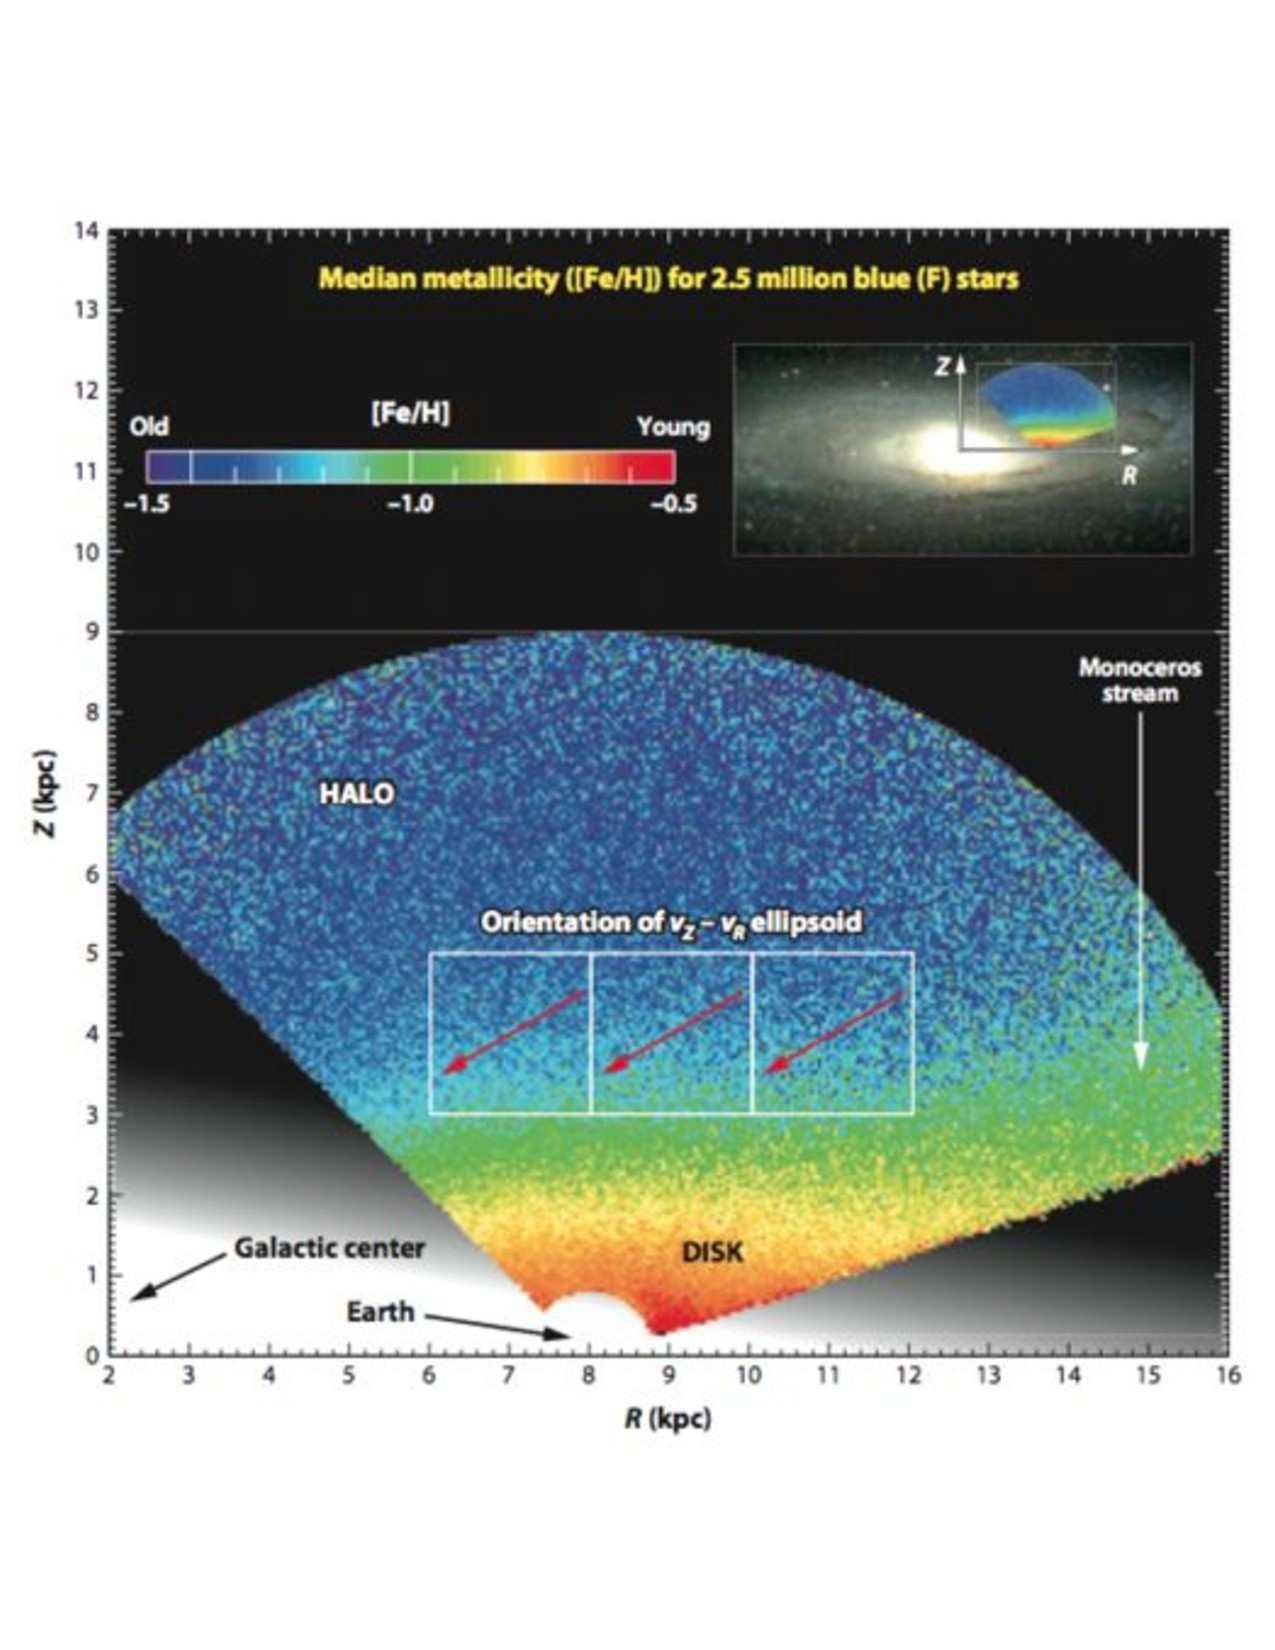
\epsfig{file=figs/IBJ_fig5.pdf, height=4.5in}
      \end{minipage} \ \hfill \
}
\end{minipage}
\vspace{-28pt}
%------------

%These recent developments, based on a host of accurate large-area surveys such as the Two-Micron All-Sky Survey \citep[2MASS;][]{2006AJ....131.1163S} and the Sloan Digital Sky Survey \citep[SDSS;][]{2000AJ....120.1579Y}, have made it abundantly clear that the Milky Way is a complex and dynamical structure that is still being shaped by the merging of smaller galaxies. Numerical simulations suggest that this merger process plays a crucial role in setting the structure and motions of stars within galaxies. Since the individual stars that make up the stellar populations in the Milky Way can be studied in great detail, their characterization proposed here will provide clues about galaxy evolution that cannot be extracted from observations of distant galaxies.
%
%To that end, I propose a two-year study to:
%\begin{itemize}
%\item mine the extensive data set provided by the Wide-Field Infrared Survey Explorer \citep[WISE;][]{2010AJ....140.1868W}, relating observables to the \emph{Spitzer} Galactic Legacy Infrared Mid-Plane Survey Extraordinaire \citep[GLIMPSE;][]{2003PASP..115..953B,2009PASP..121..213C}, SDSS, 2MASS, and other surveys.
%\item reliably identify and track a unique yet ubiquitous population of high-luminosity, IR-bright stars: Asymptotic Giant Branch (hereon AGB) stars.
%\item map the structure of the Milky Way in unprecedented detail, with AGB stars as our indicators of distance and age.
%\item use the distribution of AGB stars as observational constraints on models of the formation and evolution of the Milky Way disk.
%\end{itemize}

\section{Work Completed/In Progress}
Not since the series of SDSS tomography papers have we been able to obtain information about large scale physical and chemical characteristics of the Milky Way galaxy. Even then, the coverage of SDSS in the plane of the galaxy, and even in the galactic halo, was limited to the stripes of observation of SDSS. ALLWISE gives us the advantage of being able to observe the whole sky. And while the NIR and MIR are not immune to dust extinction along the line of sight, the influence of dust on observations is minimal as compared to optical wavelengths. 

If we're working in the NIR and Mid-IR, AGB stars are the perfect objects to serve as a proxy for structure of the Milky Way. AGB stars with dusty circumstellar shells shine brightly in the IR, with that brightness only increasing with the size of the shell. They're bright enough to be observed not only at the galactic center (even with dust extinction), but beyond out to the edge of the galactic disk. They're also ubiquitous throughout the galaxy, being the evolutionary products of low- and intermediate-mass Main Sequence stars. They have massive stellar winds that enrich their local galactic neighborhood, and their chemical content can represent the metallicity of the region in which they reside. As such, our work here is first to obtain a clean, reliable sample of these stars within the galaxy. Once obtained, we can then use the sample of ALLWISE AGB candidates in conjunction with high-confidence models of the galaxy and of the consequences of AGB star evolution to describe the Milky Way in detail, parameterized by the physical characteristics of these AGB stars.

\subsection{Development of Broad Color-Color Criteria}
We begin by selecting a known sample of AGB stars and matching to the ALLWISE-2MASS data release. The MACHO project \citep{2008AJ....136.1242F} and the Optical Gravitational Lens Experiment (OGLE) III Online Catalog of Variable Stars\footnote{\url{http://ogledb.astrouw.edu.pl/~ogle/CVS/}} both contain catalogs of AGB stars, confirmed from their variability. Additionally, the SIMBAD database\footnote{\url{http://simbad.u-strasbg.fr/simbad/}} contains objects classified as AGB stars from small surveys and individual studies. We positionally match these catalogs to objects from the ALLWISE-2MASS data using a circle of uncertainty with radius 1", and necessitate that every match have a 2MASS association.

The region of color-color space occupied by these stars is also occupied by other objects that happen to have dusty environments, as well as naked stars on the main sequence and extragalactic sources. As such, we need a reliable sample of contaminants that we can exclude in color-color space to increase the likelihood that our population of candidates represents the objects we wish to study. We gather AGN, QSOs, and star forming galaxies from the Sloan Digital Sky Survey \citep{2000AJ....120.1579Y} data release (DR) 7, specifically the NYU Value-Added Galaxy Catalog\footnote{\url{http://sdss.physics.nyu.edu/vagc/}} \citep[VAGC]{2005AJ....129.2562B}, and the LRGs from the SDSS Luminous Red Galaxy Survey \citep{2010ApJ...710.1444K}. Data for stars in the SDSS stellar locus \citep{2014MNRAS.440.3430D} were drawn from the DR 9 SEGUE Stellar Parameters Pipeline (SSPP).

\begin{figure}
% Fig 2
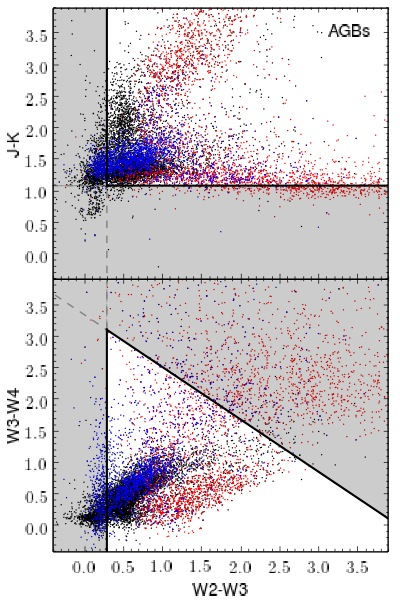
\includegraphics[width=2in]{figs/sampleboundaries.jpg}
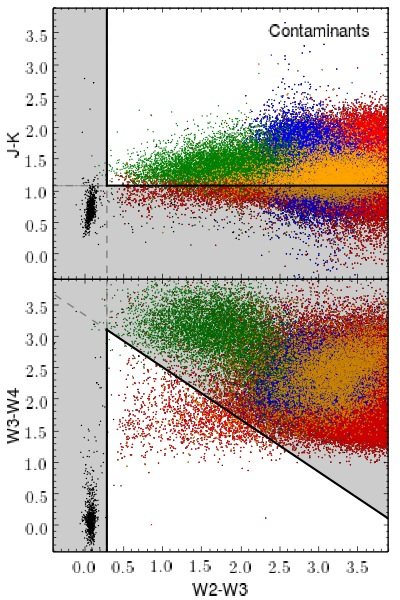
\includegraphics[width=2in]{figs/contamboundaries.jpg}
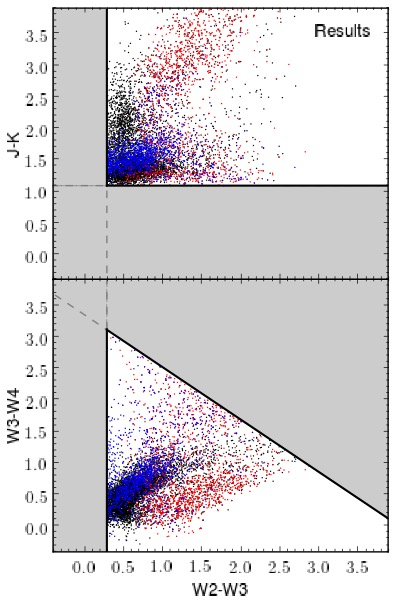
\includegraphics[width=2in]{figs/sample_results.jpg}
\caption{\emph{Left}: SIMBAD, OGLE-III, and MACHO AGB stars (black, red, blue) matched to ALLWISE within 1". \emph{Middle}: LRGs, starforming galaxies, AGN, QSO, and Locus Stars (green, red, orange, blue, black). \emph{Right}: AGB stars passing ALLWISE color criteria.}
\label{fig:boundaries}
\end{figure}

The color-color criteria set are fairly simple (Figure~\ref{fig:boundaries}), expanding upon regions in color-color space encountered in the literature. While we wish to maximize the completeness of our AGB star sample, we emphasize reliability of the sample and so minimize contamination below the 1\% level for each contaminant population and in total. We note that in our selection criteria we exclude a substantial population of AGB stars with small or non-existent circumstellar shells. This is necessary in order to also prevent stars from the stellar locus, a far more populous sample, from contaminating our candidates.

\subsection{Estimation of Distances to Candidates with {\tt GALFAST}}
%Create a sample of likely AGB star candidates and use GALFAST to estimate the dust column and distance to each candidate, using the color-color criteria of \cite{2014MNRAS.442.3361N} to differentiate between AGB stars with O-rich and C-rich atmospheres.
\begin{figure}[h]
% Fig 3
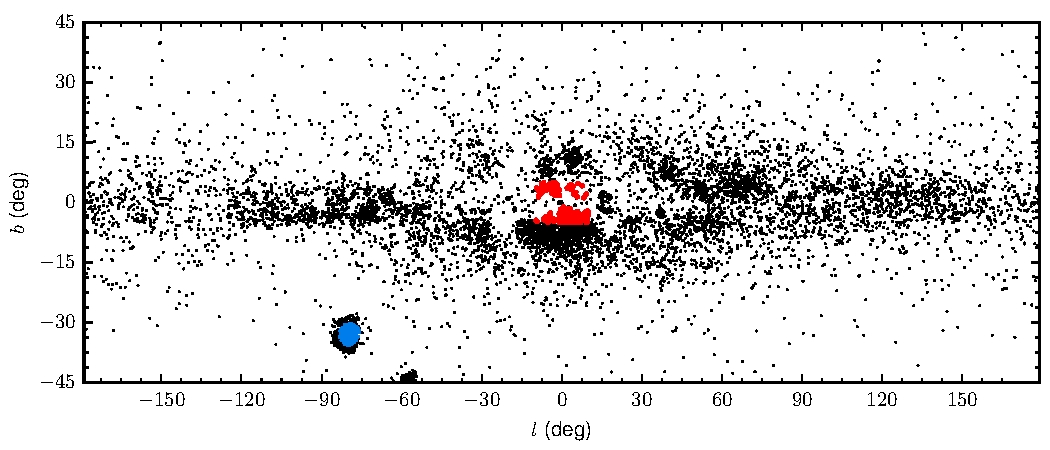
\includegraphics[width=6in]{figs/bulge_lmc_galcoords.pdf}
\caption{Galactic plot of all AGB stars passing color criteria, highlighting stars in the direction of the bulge (red) and stars in the LMC (blue).}
\label{fig:galplot}
\end{figure}

As a first step toward creating a 3D map of our galaxy using candidate AGB stars, we set out to find reliable color-magnitude relationships for our stars. From our known sample, we select objects that fit within the narrow color-color criteria for O-rich and C-rich AGB stars set by \cite{2014MNRAS.442.3361N}. We then choose stars in the direction of regions of a) known distance and b) high star concentration in order to derive our color-magnitude relationships for these stars: the Milky Way bulge and the Large Magellanic Cloud (Figure~\ref{fig:galplot}). For the LMC, we minimize foreground contamination by selecting stars with $b < -20^\circ$ and also meeting the following criteria:

$$\displaystyle\left(\frac{\text{RA} - \text{RA}_\text{LMC}}{3.5}\right)^2 + \left(\frac{\text{Dec} - \text{Dec}_\text{LMC}}{1.5} \right)^2 < 5 \text{ deg}^2.$$

\noindent With this selection of stars, we demonstrate that AGB stars possess an intrinsically-narrow magnitude distribution, as seen in \cite{1985A&A...152L...1H} and \cite{2002MNRAS.337..749J}. We however do not use this sample further to define the color-magnitude relationships for AGB stars in the IR as our {\tt GALFAST} model used for estimating the dust columns for stars doesn't include dust in or the shape of the LMC. We neglect to use the Small Magellanic Cloud entirely due to the low count of recovered objects from our initial color-color criteria.  We instead solely use the sample in the direction of the Milky Way bulge for the necessary color-magnitude calibration (Figure~\ref{fig:colormag}). We minimize the contamination from foreground stars in the direction of the Galactic bulge by selecting stars with $\lvert l\rvert < 10^\circ$, $1^\circ < \lvert b \rvert < 5^\circ$. 

\begin{figure}[h]
% Fig 4
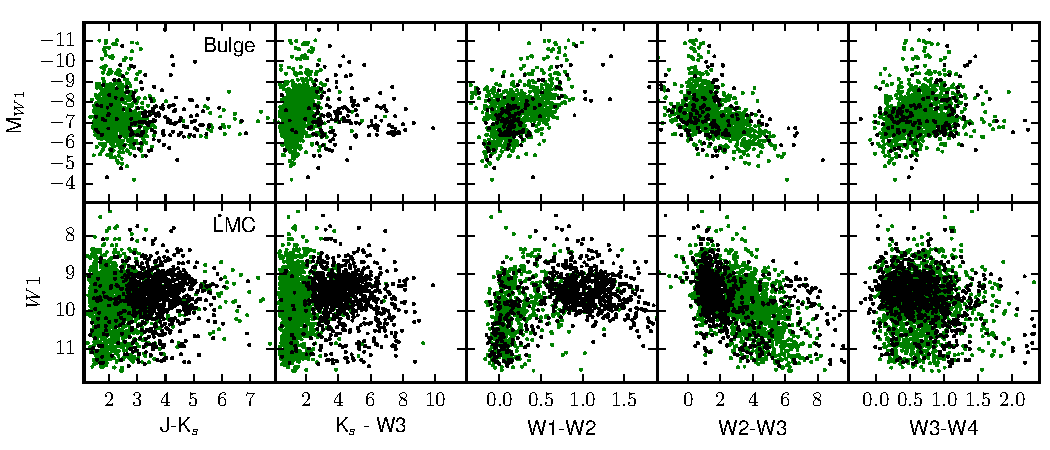
\includegraphics[width=6in]{figs/bulge_lmc_colormag.pdf}
\caption{Absolute W1 magnitude vs 2MASS-ALLWISE colors for stars in the Milky Way bulge (top) and LMC (bottom). Stars are separated into O-rich (green) and C-rich (black).}
\label{fig:colormag}
\end{figure}

Color-magnitude relations are then found for each IR color with respect to $M_{w1}$ as derived from the Milky Way bulge using linear regression. With these we estimate distances to our candidate sample to within a small degree of uncertainty ($\sim$0.5 mag).

Once a candidate sample has been retrieved from the ALLWISE-2MASS database matching our broad color criteria, we narrow them into high-photometric-quality O-rich and C-rich populations using the same criteria from \cite{2014MNRAS.442.3361N}. Assuming absolute magnitudes based upon the aforementioned color-magnitude relationships, we simultaneously estimate the distance and coefficient for dust extinction along the line of sight for each star using a convolution of the {\tt GALFAST} model and the dust maps from \cite{1998ApJ...500..525S}.

\subsection{The Milky Way in 3D and Disk Measurements}
%Create a 3D map of the galaxy using the aforementioned distances.  Measure the disk scale height as a function of radius, and the disk scale length as a function of height (if possible).
With distance information and position on the sky, we construct an X-Y-Z map of the Milky Way (Figure~\ref{fig:xyz_candidates}). We note that the overwhelming majority of AGB candidates in the Milky Way are O-rich, with the population C-rich AGB candidates of high photometric quality being essentially nonexistent, so we move forward solely with an analysis of candidates classified as such. We also note, as is clear in Figure~\ref{fig:xyz_candidates}, that this is by no means a complete picture of the Milky Way. The sample is heavily affected by dust extinction and source confusion within 0.5 kpc of the galactic disk, and entirely beyond the bulge within $|b| < 1^\circ$ of the disk. Additionally, because we exclude sources that are beyond the saturation limits of WISE, we lose a large fraction of AGB candidates near the Sun (more toward the galactic anticenter due to a lack of interstellar dust to attenuate the source's intrinsic brightness).

\begin{figure}[h]
% Fig 5
\centering
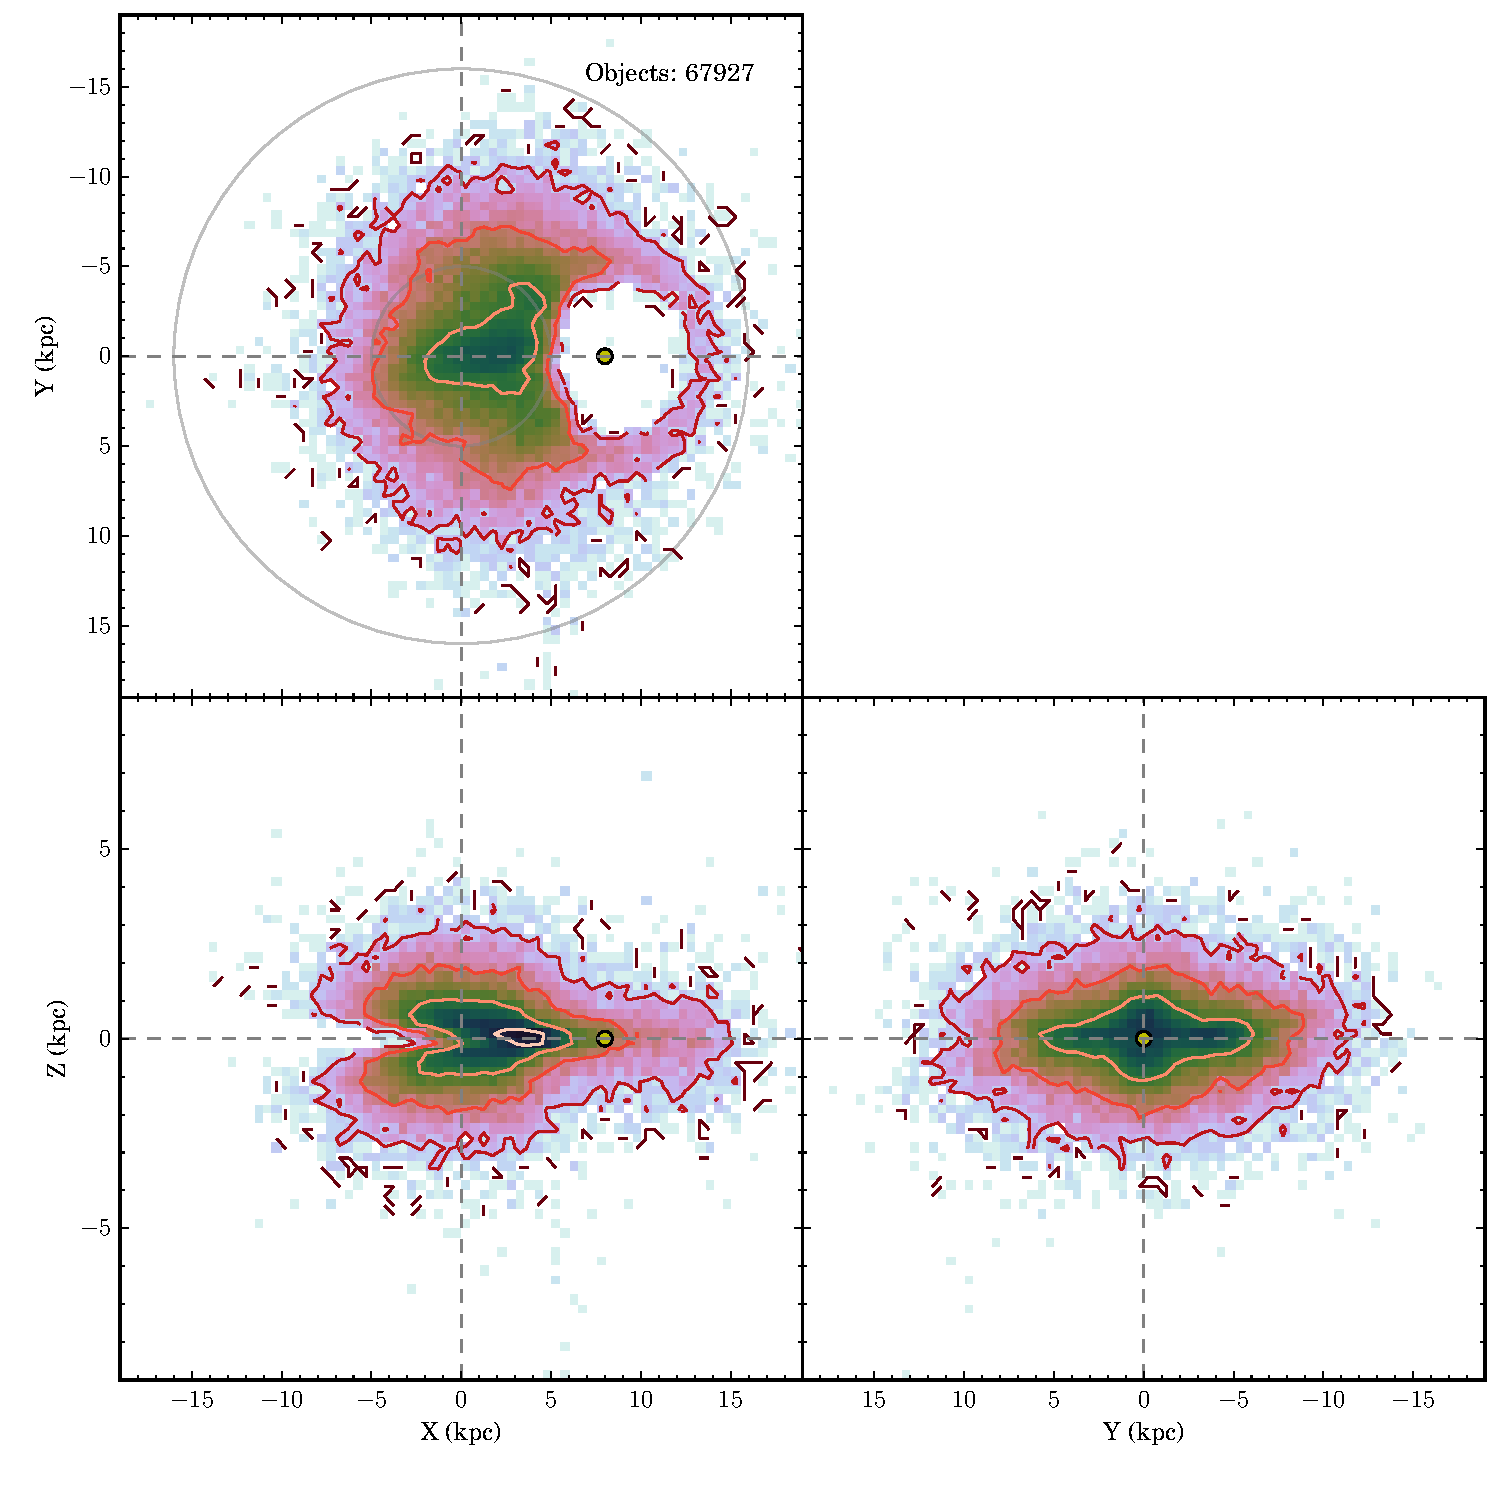
\includegraphics[width=5in]{figs/orich_candidates_xyz.pdf}
\caption{X-Y-Z distributions of the ALLWISE AGB candidate sample's O-rich stars. The Sun is set as the yellow dot with (X,Y,Z) = (8.0 kpc, 0 kpc, 0 kpc). The gray dashed lines mark (0,0) in each plot, and the contours are spaced by 0.75 logarithmically, starting at 0.}
\label{fig:xyz_candidates}
\end{figure}

Despite the loss of sources beyond the bulge and near the Sun, we are still able to make measurements of some common disk properties. We focus on the +X half of the galaxy due to the higher completeness of sources, and exclude the wedge of the Milky Way containing that solar circle. We then examine the radial and vertical distribution of AGB candidates, and derive measurements of the scale height as a function of radius, as well as the scale length as a function of height (Figure~\ref{fig:horvert_profile}).

\begin{figure}[h]
% Fig 6
\centering
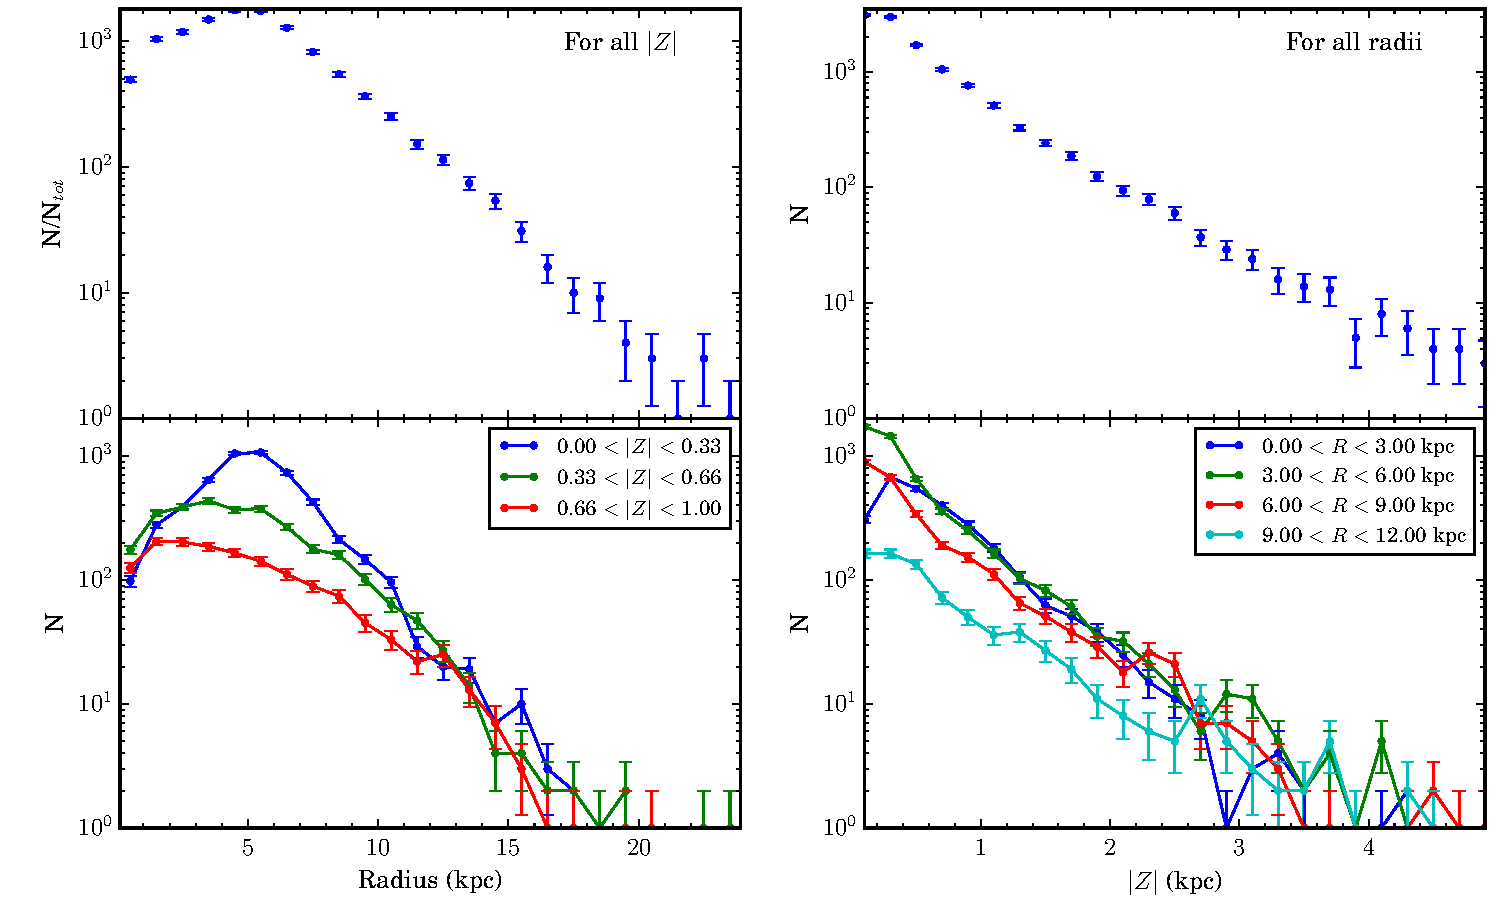
\includegraphics[width=6.5in]{figs/orich_radial_vertical_profile.pdf}
\caption{Lorem ipsum dolor sit amet, consectetur elit. Fusce, nulla rebds vel pellentesque consequat, ante nulla hendrerit arcu, ac tincidunt mauris lacus sed leo.}
\label{fig:horvert_profile}
\end{figure}

\section{Work to be Completed}
With the initial groundwork completed for the clean selection of the AGB candidate sample, dust extinction along the line of sight, and distance measurements throughout the Milky Way, we can proceed to convolve that data with high quality models of AGB star evolution and the distribution of stars throughout the Milky Way.
\subsection{Comparison with {\tt TRILEGAL}}
%Same as above, but use TRILEGAL and compare
{\tt TRILEGAL} \citep{2005A&A...436..895G, 2007ASPC..378...20G} provides us with the possibility of testing several quantities produced from the work done thus far. {\tt GALFAST} provided us with an estimation of the dust column along the line of sight to our candidate AGB stars, but with a set galactic model. {\tt TRILEGAL}  allows us to test the validity of that model, alongside several other models of the Milky Way, with respect to our now-derived 3D distribution of AGB stars by providing stellar number densities along lines of sight.

With the simulated photometry output by {\tt TRILEGAL}, along with various choices of dust chemistry used as input for these simulations, we can use our color-color information as proxies for measurements of photospheric temperature and mass-loss rate, measurements unobtainable from the photometry of ALLWISE. {\tt TRILEGAL} also has the added benefit of producing photometry for any given photometric set. Thus, we would be able to simulate photometry from the GLIMPSE survey, correlate that with photometry from ALLWISE, and use GLIMPSE photometry to fill in the population of AGB stars missing from our current sample due to source confusion and dust extinction. 

Finally, {\tt TRILEGAL} also produces estimations of stellar age, metallicity, [C/O], and periodicity. Convolved with our existing ALLWISE results and potential GLIMPSE results, we may be able to produce a 3D picture of chemical enrichment and age of the Milky Way, while also being able to see the chemical contribution of AGB stars to their local galactic neighborhoods, giving us an even fuller picture of the evolution of our galaxy.

\subsection{Derive Relations Between SDSS Stellar Properties and Position}
%Match candidate sample to APOGEE red giant survey to get actual stellar parameters as a function of position. Use above relationships to estimate circumstellar shell size, age, mass-loss rate, metallicity, anything really. Correlate that with X-Y-Z position in the galaxy (or maybe even just R-Z).
We have matched the ALLWISE AGB candidate sample to the latest results from the SDSS APOGEE survey. This provides us with actual measurements of stellar parameters that we can use to characterize our sample, as well as improve upon the existing capabilities and outputs of {\tt TRILEGAL}.

\subsection{Conclusion About Galactic Evolution w.r.t. SDSS and TRILEGAL}
%Tie the above to galactic evolution. Try to pick out large structures in the Milky Way such as the Sagittarius over density and the Monoceros Overdensities. Should at least stand out in metallicity.

\section{Timeline}
Time it takes for each bit


\vfill
\break

% References
\addcontentsline{toc}{part}{\hspace {1em}References}
\bibliographystyle{apj}
\bibliography{thesisproprefs}
\vfill
\eject



\end{document}